\begin{prob}[5]\textbf{A cvx Experiment in Compressive Sensing:}
\end{prob}
 Consider the following problem
  \begin{eqnarray*}
    \mbox{minimize} & \vert \vert x \vert \vert_{1}\\
    \mbox{subject to} & y = \Phi x
  \end{eqnarray*}
  where $\Phi$ is a $k \times n$ matrix with $k << n$, and $x$ is a vector
  with only $S$ nonzero elements. The interpretation is that $y$ constitutes
  our $k$ measurements of a sparse vector $x$, through a ``measuremnts
  matrix'' $\Phi$. Since $\Phi$ is fat, there are infinitely many vectors
  $x$ that satisfy the equality constraint in the problem, so we cannot
  determine $x$ uniquely, only from that constraint. But if know that
  $x$ is sparse (i.e., only $S$ nonzero elements of $n$), and if $k$ is
  large enough (i.e., we have enough 'projections' of $x$), then the
  optimization problem aboe can uniquely determine $x$. Note that we
  do not need to know the sparsity pattern (which elements of $x$ are
  nonzero).

  For the purposes of this problem, we will assume that $\Phi$ consists
  of rows of a DFT matrix which has an element in the $l^{th}$ row and
  $m^{th}$ column given by $[ \Phi ]_{l,m} = n^{-1/2}\exp (-j 2 \pi f_{l} m / N)$,
  where $f_{l} \in \{0,1,\ldots,n-1\}$ for $l = 1, \ldots, k$. The
  interpretation is that $x$ is being ``snsed'' or ``sampled'' in $k$
  different frequencies. Recall that $k < n$, so we have much fewer
  frequency samples than the length of $x$, hence the name compressed
  sampling or compressed sensing. An interesting result in conncetion
  with the problem above is that if $k$ frequencies are chosedn randomly
  and uniformly in the set $\{0,1,\ldots,n-1\}$, and the number of
  frequency samples are at least
  \[
  k > CS \log n
  \]
  then the above optimization problem has a solution which will reconstruct
  $x$ perfectly, with high probability. The idea is that for almost all
  selection of $k$ frequencies out of the $n$ possible, perfect reconstruction
  of the sparse $x$ is possible with much fewer than $n$, but more than
  $CS \log n$ samples, where $C$ is just some constant, independent of
  $n$ and $k$. In short, if $k$ is sufficiently large, a random selection of
  frequencies will with very high probability yield a sampling matrix
  $\Phi$ that will generate a $y$ which can be used to recover $x$ perfectly
  using the optimization problem above. This probability will approach 1 very
  rapidly expecially if $n$ is large as well. However, even when $k > CS \log n$
  is satisfied, it is possible to select the frequencies such that we
  cannot reconstruct $x$ (even though this occurs with ever smaller
  probabiliy when $n$ is large).

\begin{enumerate}[(a)]
\item{Give an example of a set of $k$ frequencies for which we would only
  be measuring a $y$ vector that would all be zeros, even though $k$ could
  be high as $n-S$ (which is clearly $> CS \log n$). To find such an
  example, think of a comb-shaped signal in discrete-time.

The measured vector $y$ will be all zeros if the following conditions are true for the parameters $n$, $S$, $k$, and the vector $x$.
\begin{itemize}
\item{The parameter $n$ is square}
\item{The number of non-zero elements in $x,S = \sqrt{n}$}
\item{The number of frequencies selected, $k = n - S = n - \sqrt{n}$}
\item{The set of frequencies selected, $\{f_{l} \in \{0, 1, \ldots, n-1\} : f_{l} \neq 0, f_{l}\neq \dfrac{pn}{S} \quad \forall \quad p \in \{1,2,\ldots\}\}$}
\item{The vector $x$ is a comb shaped function with $S$ spikes separated by $\sqrt{n}$}
\end{itemize}

An example would be:
\begin{itemize}
\item{$n = 64$}
\item{$S = \sqrt{n} = 8$}
\item{$k = n - S = 64 - 8 = 56$}
\item{$f_{1} = \{1,2, \ldots, 63, 64\}/\{8,16,24,32,40,48,56,64\}$}
\item{$x = \lbrack 0,0,0,0,0,0,0,1,0,0,0,0,0,0,0,1,\ldots\rbrack$}
\end{itemize}
  }
\item{Select $n$, $S$, and generate $\Phi$ randomly using the description
  above, where the $k$ frequencies are selected randomly, uniformly distributed
  in $\{1, 1, \ldots, n-1\}$. Use cvx to recover $x$. For values of $n=50$,
  and $n = 100$, determine the smallest value of $k$ that will recover $x$
  perfectly from randomly selected frequencies.
    different starting points.
\begin{table}[ht]
\centering
\begin{tabular}{|l|l|l|l|l|l|l|l|l|l|l|l|l|l|l|}
\hline
\multicolumn{5}{|l|}{n}                    & \multicolumn{5}{l|}{S}  & \multicolumn{5}{l|}{k}  \\ \hline
\multicolumn{5}{|l|}{\multirow{5}{*}{50}}  & \multicolumn{5}{l|}{10} & \multicolumn{5}{l|}{26} \\ \cline{6-15} 
\multicolumn{5}{|l|}{}                     & \multicolumn{5}{l|}{15} & \multicolumn{5}{l|}{33} \\ \cline{6-15} 
\multicolumn{5}{|l|}{}                     & \multicolumn{5}{l|}{25} & \multicolumn{5}{l|}{43} \\ \cline{6-15} 
\multicolumn{5}{|l|}{}                     & \multicolumn{5}{l|}{25} & \multicolumn{5}{l|}{46} \\ \cline{6-15} 
\multicolumn{5}{|l|}{}                     & \multicolumn{5}{l|}{30} & \multicolumn{5}{l|}{48} \\ \hline
\multicolumn{5}{|l|}{\multirow{5}{*}{100}} & \multicolumn{5}{l|}{20} & \multicolumn{5}{l|}{43} \\ \cline{6-15} 
\multicolumn{5}{|l|}{}                     & \multicolumn{5}{l|}{30} & \multicolumn{5}{l|}{58} \\ \cline{6-15} 
\multicolumn{5}{|l|}{}                     & \multicolumn{5}{l|}{40} & \multicolumn{5}{l|}{73} \\ \cline{6-15} 
\multicolumn{5}{|l|}{}                     & \multicolumn{5}{l|}{50} & \multicolumn{5}{l|}{90} \\ \cline{6-15} 
\multicolumn{5}{|l|}{}                     & \multicolumn{5}{l|}{60} & \multicolumn{5}{l|}{98} \\ \hline
\end{tabular}
\caption{Empircally determined values of $k$}
\label{my-label}
\end{table}

Now, table 1 presents empircally determiend values of $k$ for the perfect recovery of $x$, These $k$ values are able to recover $x$ with a fairly high precision(four positions after our decimal point) after 300 test iterations.
  }
\item{Suppose we now have noisy measurements so that $y = \Phi x + \eta$,
  where $\eta$ is an unknown noise vector that satisfies
  $\vert \vert \eta \vert \vert_{2} \leq \epsilon$. Use a $\Phi$ matrix
  and $k$ value and set of frequnecies that enable perfect recovery
  in the noiseless case to generate your data. For this data solve the following
  problem in cvx.
  \begin{eqnarray*}
    \mbox{minimize } & \vert \vert x \vert \vert_{1}\\
    \mbox{subject to } & \vert \vert y - \Phi x \vert \vert_{2} \leq \epsilon
  \end{eqnarray*}
  Plot $\vert \vert x^{*} - x \vert \vert_{2}$ versus $\epsilon$ for a
  resonable range of $\epsilon$, keeping $\Phi$, $x$ the same.
  \begin{figure}[H]
  \centering
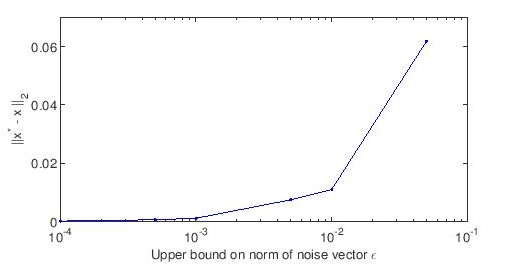
\includegraphics[width=10cm]{source/prob5/fig1}
\caption{Effet of noise on the recovery of $x$}
\end{figure}

Here we can see that as the bound of the nor of the error vecto, $\epsilon$, is increased. Then the difference between the recovered and actual value of $x$ increases.
  }
\end{enumerate}